\documentclass[11pt]{article}
\usepackage[margin=1in]{geometry}
\usepackage{fontspec}
\usepackage{amsmath,amssymb}
\usepackage{graphicx}
\usepackage{tikz}
\usepackage{booktabs}
\usepackage{array}
\usepackage{hyperref}
\usepackage{microtype}
\setmainfont{TeX Gyre Termes}
\title{Beyond Rank: Decision-Stability Radii for Multi-Task AI Leaderboards under Task Reweighting}
\author{Ghassan Malkawi*}
\date{}
\begin{document}
\maketitle
\begin{center}
\small
Faculty of Computer Information Science, Higher Colleges of Technology, Al Ain, Abu Dhabi, United Arab Emirates\\
*Corresponding author: \href{mailto:gmalkawi@hct.ac.ae}{gmalkawi@hct.ac.ae}
\end{center}

\begin{abstract}

Multi-task AI leaderboards identify a winner under a chosen aggregation, but they do not reveal how close that decision is to changing when task priorities shift. We define the decision-stability radius (DSR), an evidence-conditional measure of the minimum total-variation redistribution of task weight required to reach a specified leaderboard boundary while holding the observed score matrix fixed. We formulate DSRs for unique-winner loss, possible top-k entry, and all-competitor feasible-winner entry as linear programs with independently checked numerical witnesses. We evaluate the method on three public benchmark systems: TabArena (51 datasets × 14 methods), BenchPress (11 benchmarks × 10 models), and BeyondArena (122 complete-case datasets × 11 methods). The results reveal distinctions hidden by nominal rankings. In TabArena, TabM is the nominal runner-up, yet LightGBM is the nearest challenger to the winner boundary; RandomForest reaches the RealMLP pairwise boundary at 0.29758 but requires 0.50561 to become globally feasible. In BeyondArena, the aggregate winner changes across IID, temporal, and grouped regimes. These findings show that nominal rank, pairwise decision proximity, and global winner feasibility are distinct properties. DSR complements a leaderboard ranking by quantifying how much task priority must move before a specified decision can change.

\end{abstract}

\noindent\textbf{Keywords:} AI benchmarking; leaderboard stability; decision stability; task reweighting; sensitivity analysis; multi-criteria decision analysis

\section{Introduction}

AI leaderboards focus on a central question—who ranks first under the chosen aggregation—but they usually leave a second question unanswered: how far is that decision from changing? In a multi-task benchmark, the answer can depend on how much importance is assigned to each task. A small nominal score gap does not necessarily mean a nearby decision boundary, and the nominal runner-up need not be the model most capable of overturning the winner under reweighting. For benchmark maintainers and model selectors, rank alone therefore provides an incomplete picture of decision stability.

Existing work shows that benchmark conclusions can change with evaluation protocol (Alzahrani et al., 2024), task choice and composition (Dehghani et al., 2021; Zhang \& Hardt, 2024), benchmark redundancy (Zhang et al., 2025), preference-record perturbations (Huang et al., 2026; Oyarhoseini et al., 2026), benchmark-specific training (Gordienko et al., 2026), task-subset selection (Gusev \& Zaytsev, 2026), and sparse evaluation (Zeng \& Papailiopoulos, 2026). These studies motivate sensitivity analysis but do not answer the fixed-score question here: with the observed task-level score matrix held constant, what is the smallest redistribution of task importance that changes a specified leaderboard decision?

The contribution is deliberately narrower than general weight-sensitivity analysis, which has a long history in multi-criteria decision analysis (Mareschal, 1988; Triantaphyllou \& Sánchez, 1997; Doan \& De Smet, 2018; O’Shea et al., 2026). We adapt that sensitivity perspective to AI benchmark evidence by measuring distance to a decision boundary in total-variation units of task-weight mass, separating unique-winner loss, possible top-k entry, and all-competitor feasible-winner entry, and binding every radius to an explicit task set, candidate set, score transformation, tie rule, and nominal weight vector.

We evaluate this formulation on three public benchmark systems with different evidence structures and provide independently checkable numerical witnesses. This design tests DSR as a reusable leaderboard diagnostic rather than as a single-benchmark case study, without claiming that weight sensitivity itself is new.

\section{Related work and claim boundary}

Benchmark robustness has several meanings. Statistical methods quantify uncertainty in comparisons, aggregate metrics, or ranks (Benavoli et al., 2017; Jansen et al., 2023; Longjohn et al., 2025; Neuhof \& Benjamini, 2026; Wainer, 2023). Dataset-selection and redundancy work asks which tasks preserve rankings or capabilities (Gusev \& Zaytsev, 2026; Zhang et al., 2025), while sparse-evaluation work asks which benchmark scores can be predicted or omitted (Zeng \& Papailiopoulos, 2026).

Preference-based audits alter the observations that feed a ranking model: Huang et al. (2026) study worst-case preference deletion, Oyarhoseini et al. (2026) analyze add/drop/flip perturbations, and Gordienko et al. (2026) model benchmark-specific training. DSR instead fixes the admitted scores, task set, and candidate set and moves only continuous task-weight mass. It is therefore a deterministic distance to a declared boundary, not a probability of reversal, confidence interval, stakeholder-preference estimate, or training-manipulation cost.

The closest mathematical precedent is MCDA weight sensitivity. Wei et al. (2000) characterize weight sets compatible with preference orders in additive value models, and Doan and De Smet (2018) use inverse optimization to find weight modifications that can move an alternative to first place. A 2026 short communication by Triantaphyllou et al. identifies and corrects modeling issues in that PROMETHEE-II MILP and extends the formulation; O’Shea et al. (2026) derive precise weight-stability intervals for the weighted-sum model. We therefore do not claim a new general theory of weight sensitivity. The LPs here are derived directly for additive benchmark scores on the simplex, measure displacement in total-variation task-weight mass, separate winner, top-k, and all-competitor events, and bind each result to a declared benchmark evidence state with independently checked witnesses.

\section{Materials and methods}

\subsection{Evidence state}

To separate observed score evidence from the aggregation choice, we represent each benchmark state by a fixed task-by-method matrix and a task-weight vector. Let $D$ be the number of tasks and $M>1$ the number of methods. The lower-is-better score matrix is
\[
Z=(z_{dm})\in\mathbb{R}^{D\times M},
\]
where $z_{dm}$ is the transformed score of method $m$ on task $d$ and $z_m$ denotes column $m$. Admissible weights lie on the simplex
\[
\Delta_D=\left\{w\in\mathbb{R}^D:w_d\ge0,\ \sum_{d=1}^{D}w_d=1\right\}.
\]
The aggregate loss of method $m$ is
\[
S_m(w)=w^\top z_m,
\]
so smaller values are preferred. A nominal vector $w^0\in\Delta_D$ is fixed before sensitivity analysis; in the primary analyses, $w_d^0=1/D$ for every task $d$. Equal task weights are a transparent reference measure, not an estimate of stakeholder preferences.

The primary score representation is task-wise normalized rank with exact score ties. Let $r_{dm}$ be the average rank of method $m$ on task $d$, with rank 1 best. The transformed loss is
\[
z_{dm}=\frac{r_{dm}-1}{M-1}\in[0,1].
\]
Within-task ranks are standard for heterogeneous multi-dataset comparisons (Demšar, 2006). Because this normalization depends on the candidate pool, ranks and $M-1$ are recomputed after every method-scope change. Missing, nonnumeric, duplicate, or nonfinite values are not imputed in the primary analyses.

\subsection{Decision-stability radius}

To quantify how far the declared aggregation is from a specified decision change, let $\mathcal{B}\subseteq\Delta_D$ denote the corresponding boundary and define
\begin{equation}
\operatorname{DSR}(\mathcal{B})=\min_{w\in\mathcal{B}}\frac12\lVert w-w^0\rVert_1,
\label{eq:dsr}
\end{equation}
where $\lVert\cdot\rVert_1$ is the $L_1$ norm. Because $w$ and $w^0$ are probability vectors, DSR lies in $[0,1]$ and equals the task-weight mass reallocated from the nominal baseline. DSR $=0$ means the boundary is already reached; larger values mean more redistribution is required for that decision event.

Figure~\ref{fig:dsr-concept} summarizes the estimand: DSR moves only task weights while the admitted score matrix and evidence state remain fixed.

\begin{figure}[htbp]
\centering
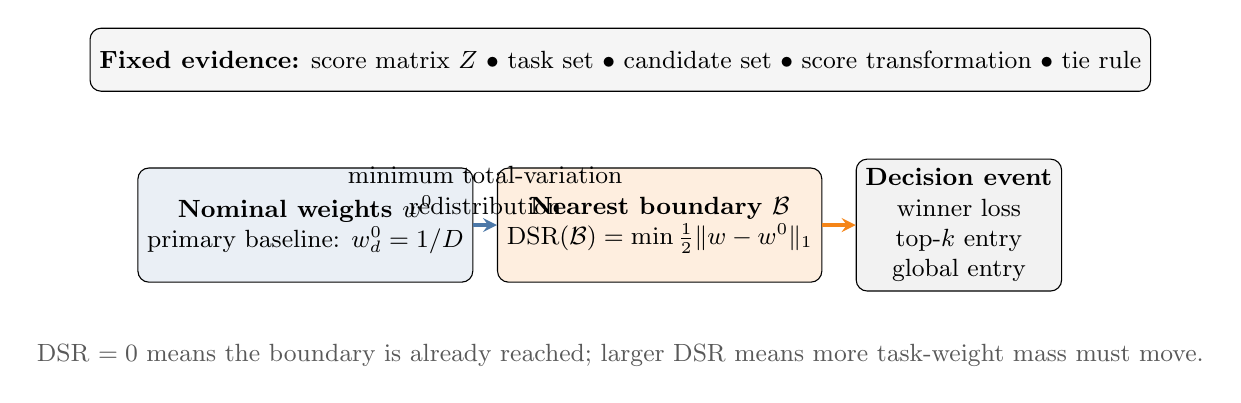
\begin{tikzpicture}[font=\small,>=stealth]
  \definecolor{pairblue}{RGB}{76,120,168}
  \definecolor{globalorange}{RGB}{245,133,24}
  \node[draw,rounded corners,fill=gray!8,minimum width=11.4cm,minimum height=0.8cm,align=center] (fixed) at (0,2.4)
  {\textbf{Fixed evidence:} score matrix $Z$ $\bullet$ task set $\bullet$ candidate set $\bullet$ score transformation $\bullet$ tie rule};
  \node[draw,rounded corners,fill=pairblue!12,minimum width=3.0cm,minimum height=1.45cm,align=center] (w0) at (-4.0,0.3)
  {\textbf{Nominal weights $w^0$}\\primary baseline: $w_d^0=1/D$};
  \node[draw,rounded corners,fill=globalorange!14,minimum width=3.5cm,minimum height=1.45cm,align=center] (b) at (0.5,0.3)
  {\textbf{Nearest boundary $\mathcal B$}\\$\operatorname{DSR}(\mathcal B)=\min \frac12\lVert w-w^0\rVert_1$};
  \node[draw,rounded corners,fill=gray!10,minimum width=2.6cm,minimum height=1.45cm,align=center] (event) at (4.3,0.3)
  {\textbf{Decision event}\\winner loss\\top-$k$ entry\\global entry};
  \draw[->,very thick,pairblue] (w0) -- node[above,align=center,text=black]{minimum total-variation\\redistribution} (b);
  \draw[->,very thick,globalorange] (b) -- (event);
  \node[align=center,text=gray!70!black] at (0,-1.35)
  {DSR $=0$ means the boundary is already reached; larger DSR means more task-weight mass must move.};
\end{tikzpicture}
\caption{Schematic of the DSR estimand. The score matrix and evidence state remain fixed; DSR is the minimum total-variation redistribution of task weight needed to reach a specified decision boundary. Schematic not to scale.}
\label{fig:dsr-concept}
\end{figure}



To ask when nominal winner $i$ can first be tied or beaten by competitor $j$, define the task-wise loss gap $g_{ij}=z_j-z_i$ and
\begin{equation}
\rho_{i\rightarrow j}=
\min_{w\in\Delta_D}\frac12\lVert w-w^0\rVert_1
\quad\text{subject to}\quad
w^\top g_{ij}\le0.
\label{eq:pairwise}
\end{equation}
The inequality is exactly $S_j(w)\le S_i(w)$. The unique-winner radius is
\begin{equation}
\rho_i=\min_{j\ne i}\rho_{i\rightarrow j}.
\label{eq:winner}
\end{equation}
Below this radius, no admitted competitor reaches the nominal winner.

Pairwise contact is not equivalent to making the challenger globally feasible. To ask when method $m$ can attain the minimum aggregate loss against the full admitted field, define
\begin{equation}
\rho_m^{\mathrm{FW}}=
\min_{w\in\Delta_D}\left\{\frac12\lVert w-w^0\rVert_1:S_m(w)\le S_\ell(w)\ \forall \ell\right\}.
\label{eq:global}
\end{equation}
If this feasible set is empty, the radius is $+\infty$. A pairwise radius against the nominal winner is therefore only a lower bound on global feasible-winner entry.

Shortlist entry is a third decision event. Let $T_k^0$ contain the $k$ methods with lowest nominal aggregate losses, assuming a strictly separated cutoff. The tie-aware possible-entry radius is
\begin{equation}
\rho_{T_k}^{\mathrm{poss}}=
\min_{\substack{a\in T_k^0\\ b\notin T_k^0}}\ 
\min_{w\in\Delta_D}\left\{\frac12\lVert w-w^0\rVert_1:S_b(w)\le S_a(w)\right\}.
\label{eq:topk}
\end{equation}
Here $a$ indexes an inside method and $b$ an outside method. The radius records the first point at which an outside method can tie or beat an inside method; a tie at the cutoff counts as possible membership. Winner, top-$k$, and global-entry radii answer different questions and need not be monotone in $k$.

\subsection{Optimization and verification}

To compute these boundaries without changing the score matrix, the absolute deviations are linearized with nonnegative auxiliary variables, yielding linear programs. Pairwise cases also have a dual program that supplies an independent optimality witness. Stored witnesses are accepted only after primal feasibility, dual feasibility, objective recomputation, primal-dual agreement, and complementary-slackness checks; global feasible-winner cases use the corresponding all-competitor constraints.

The reported LP calculations use SciPy with the HiGHS backend (Huangfu \& Hall, 2018; Virtanen et al., 2020).

The verification record contains 109 winner-versus-competitor cases across the reported scopes. Of these, 101 finite pairwise witnesses satisfy independent numerical checks; the remaining infeasible cases have explicit reasons. All 14 TabArena global feasible-winner cases satisfy the corresponding all-competitor checks, including one strict-dominance infeasibility certificate. An independently written ordered mass-transfer implementation agrees with the defining pairwise LP on 6,402 finite random validation problems, with a maximum absolute discrepancy of 1.14 × 10⁻¹³. These checks verify the numerical implementation to declared floating-point tolerances; they are not a formal proof over exact arithmetic. Supplementary Sections S1–S4 provide the detailed witness and scope traces.

\subsection{Public benchmark evidence}

We analyze three public benchmark systems.

TabArena (Erickson et al., 2025) is a living benchmark for tabular machine learning. The frozen evidence state used here contains 51 datasets and 14 complete peak-performance configurations selected under the pre-specified scope and compatibility rules preserved in the reproducibility archive. Incompatible full-suite substitutions are excluded rather than treated as observations. The resulting 51 × 14 matrix is a dated analysis state, not a claim to reproduce the continuously updated live leaderboard.

BenchPress (Zeng \& Papailiopoulos, 2026) provides a public sparse model-by-benchmark score matrix. The fixed snapshot used in this study contains 84 models, 133 benchmarks, and 2,604 observed cells (23.3\% fill). Because the DSR analysis is conditioned on observed evidence, matrix-completed predictions are not treated as observations. The primary analysis includes records whose provenance and evaluation setting could be verified, yielding a complete observed 11-benchmark × 10-model intersection. Broader source-admission rules are analyzed as scope sensitivities.

BeyondArena (Purucker et al., 2026) extends tabular evaluation beyond standard IID settings to temporal and grouped tasks. The primary fixed 11-model analysis uses 122 complete-case datasets: 97 IID, 11 temporal, and 14 grouped. Incomplete datasets are excluded rather than imputed into the primary matrix; scope-sensitivity analyses are reported separately.

The three cases are intentionally heterogeneous. TabArena tests whether point rank identifies the nearest decision boundary. BenchPress tests how evidence admission and common scope affect the analyzed decision. BeyondArena tests whether a full-suite conclusion conceals regime-specific reversals.

\section{Results}

\subsection{Primary decision-stability radii}

Table 1 summarizes the primary deterministic results. Top-3 and top-5 values are tie-aware possible-entry radii, so they need not be monotone in k. All radii remain conditional on their benchmark evidence states and should not be treated as a universal cross-benchmark scale.

\begin{table}[htbp]
\centering
\caption{Primary DSR results under the declared evidence states; top-3 and top-5 are possible-entry radii.}
\label{tab:primary}
\small
\begin{tabular}{lllll}
\toprule
Benchmark & Matrix & Nominal winner & Nearest top-1 challenger & DSR (top-1/top-3/top-5)\\
\midrule
TabArena & $51\times14$ & RealMLP & LightGBM & 0.03660 / 0.02832 / 0.00545\\
BenchPress & $11\times10$ & Claude Opus 4.6 & GPT-5.2 & 0.09091 / 0.04091 / 0.17172\\
BeyondArena & $122\times11$ & TabPFN-2.6 & TabICLv2 & 0.01867 / 0.08607 / 0.01892\\
\bottomrule
\end{tabular}
\end{table}

\subsection{Nominal rank is not decision proximity}

In TabArena, RealMLP is the nominal winner and TabM is second in the nominal ordering. However, LightGBM is the nearest winner-boundary challenger, with top-1 DSR 0.0366013072. The runner-up is therefore not the model closest to removing the unique-winner conclusion.

Shortlist stability differs again. The top-3 possible-entry radius is 0.0283224401, where CatBoost can enter by displacing TabM before RealMLP loses its unique-winner status. The top-5 radius is 0.0054466231, where XGBoost can enter by displacing ModernNCA. Thus nominal rank, winner stability, and shortlist stability are not interchangeable summaries.

\subsection{Pairwise contact does not imply global winner feasibility}

A challenger can tie the nominal winner while still being beaten by another method. In TabArena, LightGBM and TabM become globally feasible at their pairwise boundaries, but several later candidates require additional task-weight movement.

The clearest example is RandomForest. It reaches the RealMLP pairwise boundary at 0.29758, yet its global feasible-winner radius is 0.50561, a gap of 0.20804 before rounding. XGBoost similarly has pairwise radius 0.14542 and global-entry radius 0.22540. KNN cannot be a global winner for any admissible task-weight vector because it is strictly dominated task-wise. These cases show why a pairwise robustness number cannot generally substitute for an all-competitor feasibility analysis; Figure~\ref{fig:pairwise-global} makes the separation explicit.

\begin{figure}[htbp]
\centering
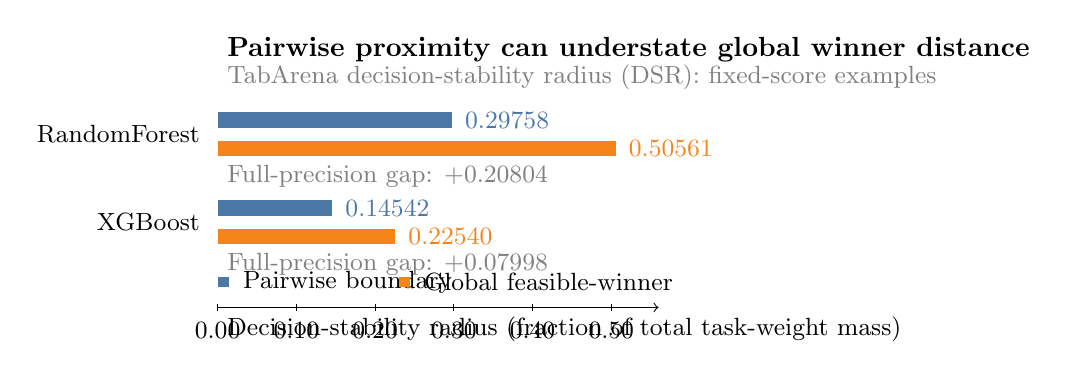
\begin{tikzpicture}[x=10cm,y=0.8cm,font=\small]
  \definecolor{pairblue}{RGB}{76,120,168}
  \definecolor{globalorange}{RGB}{245,133,24}

  \node[anchor=west,font=\bfseries] at (0,4.5) {Pairwise proximity can understate global winner distance};
  \node[anchor=west,text=gray] at (0,4.05) {TabArena decision-stability radius (DSR): fixed-score examples};

  \draw[->] (0,0.4) -- (0.56,0.4);
  \foreach \x/\lab in {0/0.00,0.1/0.10,0.2/0.20,0.3/0.30,0.4/0.40,0.5/0.50}
    {\draw (\x,0.35)--(\x,0.45) node[below=3pt] {\lab};}

  \node[anchor=east] at (-0.01,3.15) {RandomForest};
  \fill[pairblue] (0,3.25) rectangle (0.29758,3.50);
  \fill[globalorange] (0,2.80) rectangle (0.50561,3.05);
  \node[anchor=west,text=pairblue] at (0.302,3.375) {0.29758};
  \node[anchor=west,text=globalorange] at (0.510,2.925) {0.50561};
  \node[anchor=west,text=gray] at (0,2.48) {Full-precision gap: +0.20804};

  \node[anchor=east] at (-0.01,1.75) {XGBoost};
  \fill[pairblue] (0,1.85) rectangle (0.14542,2.10);
  \fill[globalorange] (0,1.40) rectangle (0.22540,1.65);
  \node[anchor=west,text=pairblue] at (0.150,1.975) {0.14542};
  \node[anchor=west,text=globalorange] at (0.230,1.525) {0.22540};
  \node[anchor=west,text=gray] at (0,1.08) {Full-precision gap: +0.07998};

  \fill[pairblue] (0,0.72) rectangle (0.015,0.88);
  \node[anchor=west] at (0.02,0.80) {Pairwise boundary};
  \fill[globalorange] (0.23,0.72) rectangle (0.245,0.88);
  \node[anchor=west] at (0.25,0.80) {Global feasible-winner};

  \node[anchor=west] at (0,0.05) {Decision-stability radius (fraction of total task-weight mass)};
\end{tikzpicture}
\caption{Pairwise versus global feasible-winner decision-stability radii for two TabArena challengers. Global feasibility can require additional task-weight redistribution beyond pairwise contact with the nominal winner. Endpoint labels are rounded; gap annotations use the stored full-precision radii.}
\label{fig:pairwise-global}
\end{figure}



\subsection{Full-suite aggregation can conceal regime-specific reversals}

For the fixed 11-model, 122-dataset BeyondArena analysis, TabPFN-2.6 is the equal-dataset winner and TabICLv2 is the nearest challenger; the top-1 DSR is 0.0186703097.

The winner is not common across the published task regimes. On the 97 IID datasets, TabICLv2 is the aggregate winner with top-1 DSR 0.0057274. On the 11 temporal datasets, TabPFN-2.6 wins with DSR 0.102273. On the 14 grouped datasets, RealMLP wins with DSR 0.0714286. A regime-balanced baseline assigning one-third of total task weight to each regime changes the all-dataset winner to RealMLP and yields top-1 DSR 0.0051179.

Figure~\ref{fig:beyond-regimes} summarizes the regime dependence: both the winner identity and the top-1 DSR change across the full-suite, IID, temporal, grouped, and regime-balanced analyses.

\begin{figure}[htbp]
\centering
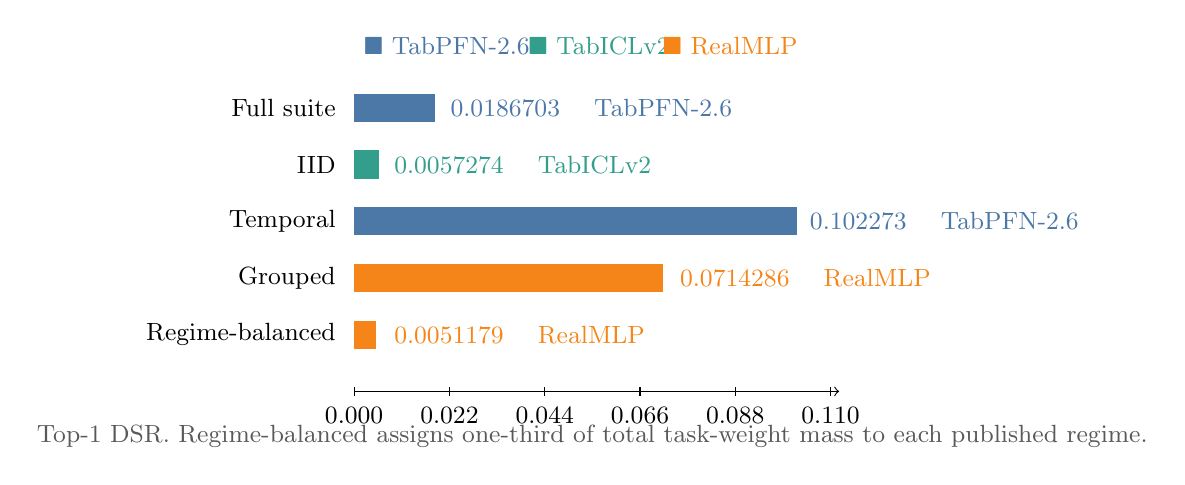
\begin{tikzpicture}[x=55cm,y=0.72cm,font=\small]
  \definecolor{tabpfn}{RGB}{76,120,168}
  \definecolor{tabicl}{RGB}{51,158,140}
  \definecolor{realmlp}{RGB}{245,133,24}
  \draw[->] (0,0) -- (0.112,0);
  \foreach \x/\lab in {0/0.000,0.022/0.022,0.044/0.044,0.066/0.066,0.088/0.088,0.110/0.110}
    {\draw (\x,-0.08)--(\x,0.08) node[below=4pt] {\lab};}
  \node[anchor=east] at (-0.002,5) {Full suite};
  \fill[tabpfn] (0,4.75) rectangle (0.0186703097,5.25);
  \node[anchor=west,text=tabpfn] at (0.020,5) {0.0186703 \quad TabPFN-2.6};
  \node[anchor=east] at (-0.002,4) {IID};
  \fill[tabicl] (0,3.75) rectangle (0.0057274,4.25);
  \node[anchor=west,text=tabicl] at (0.007,4) {0.0057274 \quad TabICLv2};
  \node[anchor=east] at (-0.002,3) {Temporal};
  \fill[tabpfn] (0,2.75) rectangle (0.102273,3.25);
  \node[anchor=west,text=tabpfn] at (0.103,3) {0.102273 \quad TabPFN-2.6};
  \node[anchor=east] at (-0.002,2) {Grouped};
  \fill[realmlp] (0,1.75) rectangle (0.0714286,2.25);
  \node[anchor=west,text=realmlp] at (0.073,2) {0.0714286 \quad RealMLP};
  \node[anchor=east] at (-0.002,1) {Regime-balanced};
  \fill[realmlp] (0,0.75) rectangle (0.0051179,1.25);
  \node[anchor=west,text=realmlp] at (0.007,1) {0.0051179 \quad RealMLP};
  \node[anchor=west,text=tabpfn] at (0,6.1) {$\blacksquare$ TabPFN-2.6};
  \node[anchor=west,text=tabicl] at (0.038,6.1) {$\blacksquare$ TabICLv2};
  \node[anchor=west,text=realmlp] at (0.069,6.1) {$\blacksquare$ RealMLP};
  \node[align=center,text=gray!70!black] at (0.055,-0.8)
  {Top-1 DSR. Regime-balanced assigns one-third of total task-weight mass to each published regime.};
\end{tikzpicture}
\caption{BeyondArena top-1 DSR and nominal winner across the full-suite, IID, temporal, grouped, and regime-balanced analyses. The regime-balanced baseline assigns one-third of total task-weight mass to each published regime.}
\label{fig:beyond-regimes}
\end{figure}



These results do not imply that one regime is the correct benchmark. They show that a full-suite winner is conditional on the distribution of task mass across structurally different evaluation regimes.

\subsection{Evidence admission changes the decision being analyzed}

Under the primary BenchPress admission rule, the complete-case analysis contains 10 models and 11 benchmarks. Claude Opus 4.6 is the nominal winner, GPT-5.2 is the nearest challenger, and the top-1 DSR is 1/11 = 0.0909090909. At the nearest boundary, the optimal reweighting transfers one equal benchmark-weight unit from MMLU-Pro to AIME 2025.

Broader source-admission rules expand the common benchmark scope. Adding third-party records whose provenance and evaluation setting could be checked yields a 10-model × 12-benchmark scope with top-1 DSR 0.1250; admitting all released source categories yields a 10-model × 13-benchmark scope with DSR 0.14103. In a fixed 10-model × 11-benchmark control, the admitted cell values, winner, and radius remain unchanged across the three source rules. The observed differences are therefore associated with admission-and-scope expansion in this snapshot, not identified as a source-class causal effect.

\section{Discussion}

The central empirical result is that a point leaderboard does not fully describe the geometry of its decision. The nominal runner-up need not be the nearest model capable of overturning the winner; a top-k set can change before the winner changes; and a model that reaches the current winner pairwise may remain infeasible against the rest of the field.

DSR is useful because its unit has a direct interpretation. A radius of 0.04 means that four percentage points of total task-weight mass must be redistributed from the nominal vector to reach the specified boundary. This interpretation is more transparent than treating a raw nominal score gap as a universal measure of robustness. It also makes the decision event explicit: winner DSR, top-k DSR, and global feasible-winner DSR are different quantities.

The results also show why evidence governance belongs inside the analysis rather than in an appendix. BenchPress is sparse; changing the admission rule changes the common model-benchmark intersection. BeyondArena contains distinct IID, temporal, and grouped regimes whose aggregate winners differ. TabArena is a living benchmark whose candidate and configuration scope can evolve. A DSR without a dated evidence state would therefore be underspecified.

The method complements rather than replaces statistical uncertainty analysis. Resampling asks how outcomes vary under a sampling model; DSR asks how far declared task priorities must move inside a fixed admitted matrix. These quantities answer different questions and should not be interpreted as substitutes.

The work also differs from strategic benchmark manipulation. Gordienko et al. (2026) ask how many datasets would need benchmark-specific training to promote a target model. Here model scores are held fixed and only the declared aggregation weights move. Likewise, Gusev and Zaytsev (2026) study task subsets that preserve rankings, whereas DSR measures distance to a specified boundary under a fixed task set.

A useful reporting practice follows from these distinctions. A leaderboard that uses weighted aggregation should report, alongside the point ranking, the nominal weights, candidate and task scope, score transformation, tie rule, top-1 DSR, and—when model selection is important—top-k and global feasible-winner radii. Such reporting does not declare a benchmark “robust” or “fragile” in the abstract; it states how far a particular decision is from a particular boundary.

\section{Limitations}

The analysis is conditional on fixed observed score matrices. It does not model adaptive benchmark overfitting, strategic retraining after protocol disclosure, causal effects of benchmark design, or unobserved evaluation errors. Equal task weights are a declared baseline rather than a claim that all tasks are substantively equally important.

Task-wise rank normalization makes heterogeneous metrics comparable but discards cardinal performance magnitude and depends on the candidate pool. We therefore fix candidate scope before ranking and treat min-max normalization only as a sensitivity analysis. Adding or removing a model can change normalized ranks even when retained raw scores do not change.

No-imputation protects the distinction between observed and predicted evidence, but complete-case analysis can be selective. This is particularly important for BenchPress and BeyondArena. The declared scope-sensitivity analyses expose this dependence but do not make missingness ignorable.

Radii from different benchmark matrices should not be read as a universal league table of benchmark robustness. A DSR is conditional on the task set, candidate set, transformation, nominal weights, and tie semantics of its evidence state.

Finally, the numerical witnesses are verified to declared floating-point tolerances. Independent code paths reduce implementation risk but do not constitute formal verification in rational or interval arithmetic.

\section{Conclusions}

The decision-stability radius turns leaderboard sensitivity into a decision-specific distance: the amount of task-weight mass that must move before a declared conclusion can change.

Across three public benchmark systems, the evidence establishes three distinctions that a point ranking alone does not show. The nominal runner-up need not be the nearest challenger; pairwise contact with the winner need not make a model globally feasible; and the reported decision can depend on the admitted task regime and evidence scope. The TabArena RandomForest result—0.29758 to reach the pairwise boundary versus 0.50561 to become globally feasible—shows why these decision events should not be conflated.

The practical implication is straightforward: multi-task leaderboards should report not only point rankings, but also the evidence state and a decision-specific stability radius. DSR is not a universal robustness score; it is a reproducible measure of how far a stated leaderboard conclusion lies from changing under task reweighting. Reporting rank without its decision distance can therefore hide how conditional the conclusion is to the benchmark’s declared task priorities.

\section*{Acknowledgments}

The author acknowledges the institutional support of the Higher Colleges of Technology, United Arab Emirates.

\section*{Conflict of interest}

The author has no conflict of interest to declare.

\section*{Funding}

The author received no specific funding for this work.

\section*{Data availability}

The analyses use publicly available benchmark and result artifacts cited in the manuscript. The public project repository, including the current manuscript and supplementary sources plus machine-readable evidence-state and result summaries, is available at \url{https://github.com/shaikhamalkawi-ux/Decision-Stability-in-Multi-Task-AI-Leaderboards-Verified-Boundaries-under-Task-Reweighting}. Third-party raw artifacts are not redistributed where redistribution status is unclear; source identities and retrieval metadata are recorded instead.

\section*{Author contributions}

Ghassan Malkawi: conceptualization, methodology, investigation, validation, writing—original draft, writing—review and editing, and supervision. The author reviewed and approved the manuscript and agrees to its submission.

\section*{Declaration of generative AI and AI-assisted technologies}

During preparation of this work, the author used OpenAI ChatGPT and Codex for language editing, code drafting, literature-search assistance, document organization, and preparation support under direct author supervision. The author reviewed the mathematical specification, source-admission decisions, calculations, evidence classifications, references, and interpretations and takes responsibility for the manuscript.

\begin{thebibliography}{99}

\bibitem{ref1} Alzahrani, N., Alyahya, H., Alnumay, Y., AlRashed, S., Alsubaie, S., Almushayqih, Y., Mirza, F., Alotaibi, N., Al-Twairesh, N., Alowisheq, A., Bari, M. S., \& Khan, H. (2024). When benchmarks are targets: Revealing the sensitivity of large language model leaderboards. Proceedings of the 62nd Annual Meeting of the Association for Computational Linguistics, 13787–13805. doi:10.18653/v1/2024.acl-long.744

\bibitem{ref2} Benavoli, A., Corani, G., Demšar, J., \& Zaffalon, M. (2017). Time for a change: A tutorial for comparing multiple classifiers through Bayesian analysis. Journal of Machine Learning Research, 18(77), 1–36.

\bibitem{ref3} Dehghani, M., Tay, Y., Gritsenko, A. A., Zhao, Z., Houlsby, N., Diaz, F., Metzler, D., \& Vinyals, O. (2021). The benchmark lottery. arXiv:2107.07002. doi:10.48550/arXiv.2107.07002

\bibitem{ref4} Demšar, J. (2006). Statistical comparisons of classifiers over multiple data sets. Journal of Machine Learning Research, 7, 1–30.

\bibitem{ref5} Doan, N. A. V., \& De Smet, Y. (2018). An alternative weight sensitivity analysis for PROMETHEE II rankings. Omega, 80, 166–174. doi:10.1016/j.omega.2017.08.017

\bibitem{ref6} Erickson, N., Purucker, L., Tschalzev, A., Holzmüller, D., Desai, P. M., Salinas, D., \& Hutter, F. (2025). TabArena: A living benchmark for machine learning on tabular data. Advances in Neural Information Processing Systems, 38, 17285–17350. doi:10.52202/085713-0519

\bibitem{ref7} Gordienko, P., Schollmeyer, G., Kreuter, F., \& Jansen, C. (2026). How hard is it to rig a benchmark? A social choice analysis of leaderboard robustness. arXiv:2605.23628.

\bibitem{ref8} Gusev, R., \& Zaytsev, A. (2026). Benchmarking on tasks that matter: Dataset selection for preserving model rankings. Proceedings of the 32nd ACM SIGKDD Conference on Knowledge Discovery and Data Mining V.2, 8954–8965. doi:10.1145/3770855.3817569

\bibitem{ref9} Huang, J. Y., Shen, Y., Wei, D., \& Broderick, T. (2026). Dropping just a handful of preferences can change top large language model rankings. International Conference on Learning Representations (ICLR 2026).

\bibitem{ref10} Huangfu, Q., \& Hall, J. A. J. (2018). Parallelizing the dual revised simplex method. Mathematical Programming Computation, 10(1), 119–142. doi:10.1007/s12532-017-0130-5

\bibitem{ref11} Jansen, C., Nalenz, M., Schollmeyer, G., \& Augustin, T. (2023). Statistical comparisons of classifiers by generalized stochastic dominance. Journal of Machine Learning Research, 24(231), 1–37.

\bibitem{ref12} Longjohn, R., Gopalan, G., \& Casleton, E. (2025). Statistical uncertainty quantification for aggregate performance metrics in machine learning benchmarks. arXiv:2501.04234.

\bibitem{ref13} Mareschal, B. (1988). Weight stability intervals in multicriteria decision aid. European Journal of Operational Research, 33(1), 54–64. doi:10.1016/0377-2217(88)90254-8

\bibitem{ref14} Neuhof, B., \& Benjamini, Y. (2026). Rank intervals for leaderboards: A hierarchical framework for model evaluation. arXiv:2606.08679.

\bibitem{ref15} O’Shea, R., Deeney, P., Triantaphyllou, E., Diaz-Balteiro, L., \& Tarim, S. A. (2026). Weight stability intervals for multi-criteria decision analysis using the weighted sum model. Expert Systems with Applications, 296, 128460. doi:10.1016/j.eswa.2025.128460

\bibitem{ref16} Oyarhoseini, H., Lin, J., \& Karimi, A.-H. (2026). A unified perturbation framework for analyzing leaderboard stability and manipulation. arXiv:2605.15761.

\bibitem{ref17} Purucker, L., Tschalzev, A., Erickson, N., Blayer, G., Holzmüller, D., Arazi, A., Pfefferle, A., Tajjar, M., Varoquaux, G., \& Hutter, F. (2026). Beyond IID: How general are tabular foundation models, really? arXiv:2606.30410.

\bibitem{ref18} Triantaphyllou, E., O’Shea, R., De Smet, Y., \& Doan, N. A. V. (2026). A communication on the paper “An alternative weight sensitivity analysis for PROMETHEE II rankings”. Omega, 140, 103465. doi:10.1016/j.omega.2025.103465

\bibitem{ref19} Triantaphyllou, E., \& Sánchez, A. (1997). A sensitivity analysis approach for some deterministic multi-criteria decision-making methods. Decision Sciences, 28(1), 151–194. doi:10.1111/j.1540-5915.1997.tb01306.x

\bibitem{ref20} Virtanen, P., Gommers, R., Oliphant, T. E., et al. (2020). SciPy 1.0: Fundamental algorithms for scientific computing in Python. Nature Methods, 17(3), 261–272. doi:10.1038/s41592-019-0686-2

\bibitem{ref21} Wainer, J. (2023). A Bayesian Bradley–Terry model to compare multiple ML algorithms on multiple data sets. Journal of Machine Learning Research, 24(341), 1–34.

\bibitem{ref22} Wei, Q.-L., Ma, J., \& Fan, Z.-P. (2000). A parameter analysis method for the weight-set to satisfy preference orders of alternatives in additive multi-criteria value models. Journal of Multi-Criteria Decision Analysis, 9(5), 181–190. doi:10.1002/1099-1360(200009)9:5<181::AID-MCDA275>3.0.CO;2-B

\bibitem{ref23} Zeng, Y., \& Papailiopoulos, D. (2026). You don’t need to run every eval. arXiv:2606.24020.

\bibitem{ref24} Zhang, G., \& Hardt, M. (2024). Inherent trade-offs between diversity and stability in multi-task benchmarks. Proceedings of the 41st International Conference on Machine Learning, 235, 58984–59002.

\bibitem{ref25} Zhang, Z., Zhao, X., Fang, X., Li, C., Liu, X., Min, X., Duan, H., Chen, K., \& Zhai, G. (2025). Redundancy principles for MLLMs benchmarks. Proceedings of the 63rd Annual Meeting of the Association for Computational Linguistics, 12492–12504. doi:10.18653/v1/2025.acl-long.612

\end{thebibliography}

\end{document}
